\documentclass{article}

\usepackage{graphicx}

\begin{document}
	\section*{Lab1 - Filip Jędrzejewski}
	
	\subsection*{Zadanie 1}
	W zadaniu należało wyznaczyć przybliżoną wartość pochodnej w punkcie za pomocą wzorów:
	
	\begin{equation}
	f'(x) = \frac{f(x+h)-f(x)}{h}
	\end{equation}
	
	\begin{equation}
	f'(x) = \frac{f(x+h)-f(x-h)}{2h}
	\end{equation}
	
	Badana funkcja:
	
	\begin{equation}
	f(x) = \tan (x)
	\end{equation}
	
	Pochodna funkcji $f(x)$ ma postać:
	
	\begin{equation}
	f'(x) = \sec ^2 (x) = 1+\tan ^ 2 (x)
	\end{equation}
	
	Funkcje badano dla argumentu:
	
	$$x = 1$$
	
	Na podstawie wzorów (1) i (2) wykonano wykresy wartości bezwzględnej błędu w zależności od wartości $h = 10^{-k}$, przy czym: $k = 0,1,2,3,...,16$. Osie są w skali logarytmicznej.
	
	\begin{figure}[h]
    		\centering
  		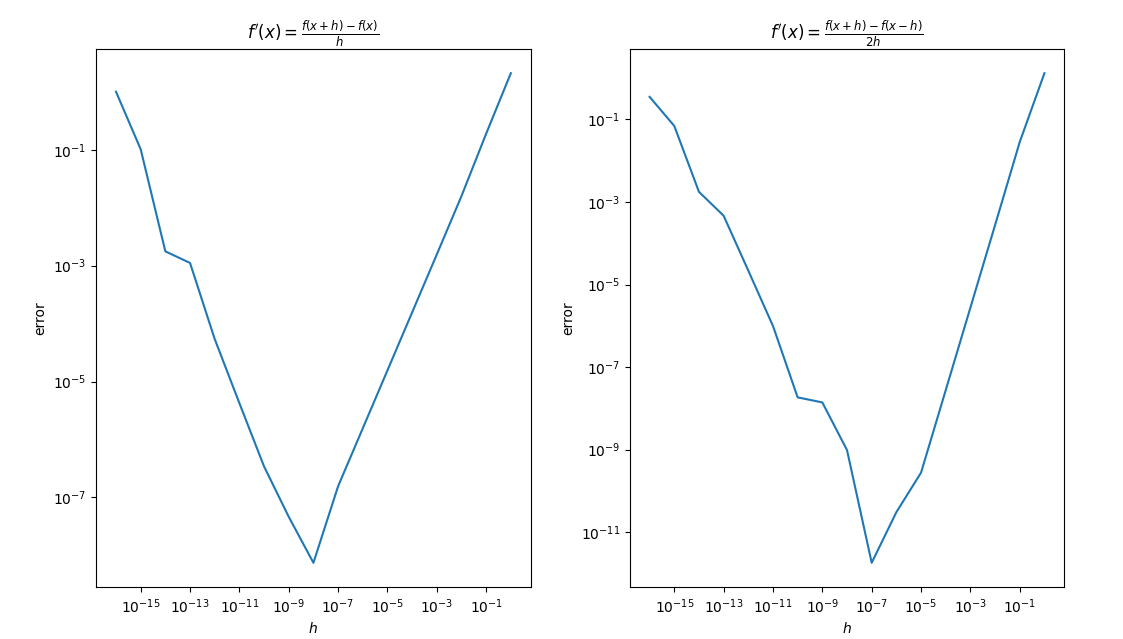
\includegraphics[scale = 0.5]{zad1.png}
	\end{figure}
	
	Wykresy wartości bezwzględnych błędów mają swoje minima dla wartości $h_{min}$ odpowiednio:
	
	$$h_{min_1} = 10^{-8}$$
	$$h_{min_2} = 10^{-7}$$
	
	Wartość $h_{min}$ obliczono również ze wzoru:
	
	\begin{equation}
		h_{min} \approx \sqrt{\varepsilon_{mach}}
	\end{equation}
	
	Otrzymana wartość:
	
	$$h_{min} \approx 1.4901161193847656 \cdot 10^{-8} \approx 1.49 \cdot 10^{-8}$$
	
	Wartość pochodnej funkcji $f(x) = \tan (x)$ dla argumentu $x = 1$ obliczonej za pomocą wzoru (1) posiadała najmniejszy błąd dla $h_{min_1} = 10^{-8}$. Jest to wartość bardzo zbliżona do teoretycznej wartości wyznaczonej za pomocą zależności (5). \newline \newline
	Wartość pochodnej tej samej funkcji przybliżana za pomocą wzoru różnic centralnych - zależność (2), przyjmowała wartość najmniejszą dla $h_{min_2} = 10^{-7}$. Jest ona prawie dziesięciokrotnie większa od teoretycznej $h_{min} = 1.49 \cdot 10^{-8}$. 
	
	\newline
	
	
	\subsection*{Zadanie 2}
	
	W zadaniu należało wygenerować pierwsze $225$ wyrazów ciągu danego wzorem:
	
	\begin{equation}
		x_{k+1} = 2.25 \cdot x_k - 0.5 \cdot x_{k-1}	
	\end{equation}
	
	Powyższy wzór przekształcono:
	
	\begin{equation}
		a_n = 2.25 \cdot a_{n-1} - 0.5 \cdot a_{n-2}
	\end{equation}
	
	Z wyrazami początkowymi:
	
	$$a_1 = \frac{1}{3}$$
	
	$$a_2 = \frac{1}{12}$$
	
	Dokładnym rozwiązaniem równania różnicowego jest:
	
	\begin{equation}
		a_n = \frac{4^{1-n}}{3}
	\end{equation}
	
	Na podstawie wzoru (7) wyznaczono iteracyjnie pierwsze $225$ wyrazów ciągu $a_n$. Następnie dla każdego obliczonego wyrazu tego ciągu obliczono błąd względny za pomocą zależności:
	
	\begin{equation}
		error = \frac{| a_n - true_{a_n} |}{true_{a_n}}
	\end{equation}
	
	przy czym: \\ 
	$error$ - obliczana wartość błędu względnego,  \\
	$a_n$ - n-ty wyraz ciągu wyznaczony za pomocą zależności (7), \\
	$true_{a_n}$ - wartość n-tego wyrazu ciągu wyznaczona za pomocą wzoru (8).
	\newline
	\newline
	
	W kolejnym kroku wykonano wykresy wartości wyrazów ciągu oraz odpowiadających im błędów względnych w zależności od $n$ (osie $y$ obu wykresów są w skali logarytmicznej).
	
	\begin{figure}[h]
    		\centering
  		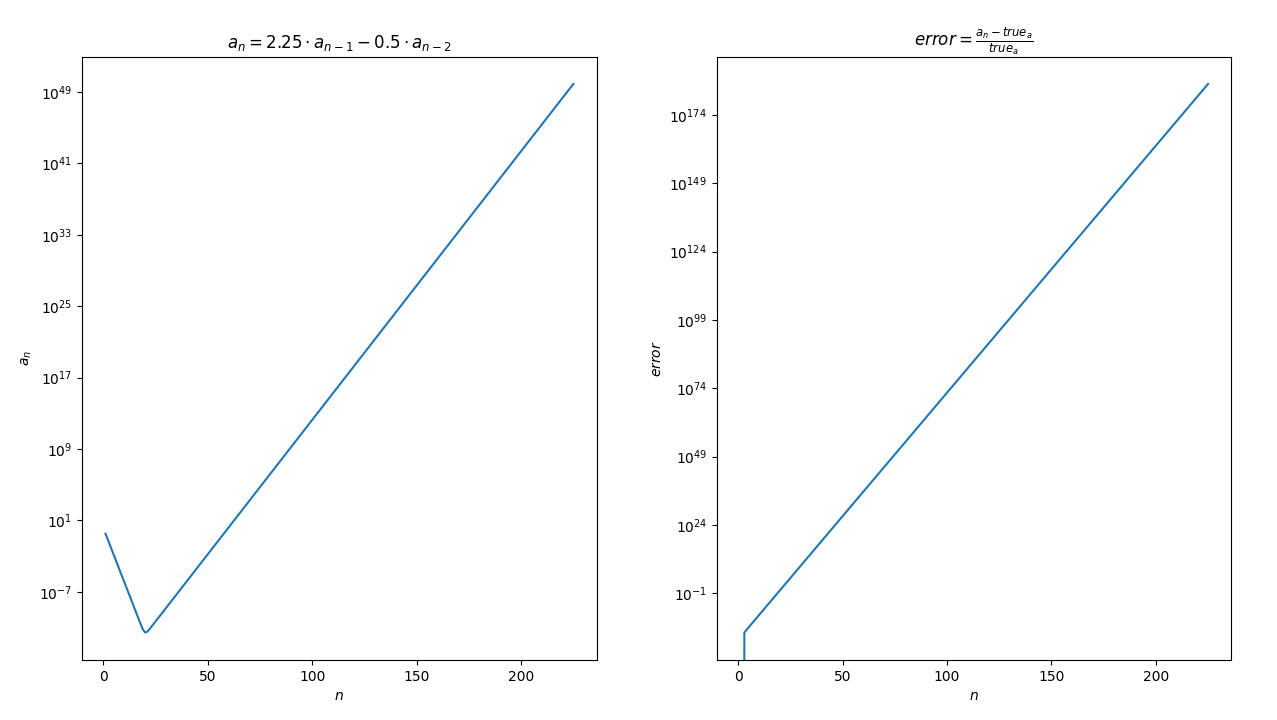
\includegraphics[scale = 0.5]{zad2.png}
	\end{figure}
	
	Dokładne rozwiązania równania - wzór (8), wskazuje na to, że ciąg jest malejący. Na wykresie wyraźnie widać, że wyznaczone wartości kolejnych wyrazów gwałtownie rosną. Wraz ze wzrostem wyrazów rośnie również błąd względny. \newline \newline
	Wykres ciągu $a_n$ zaczyna rosnąć od 20-tego wyrazu, dla którego przyjmuje minimum równe:
	
	$$a_{20} \approx 2.771793376831781 \cdot 10^{-12} \approx 2.77 \cdot 10^{-12}$$
	
	Jest to zatem bardzo mała liczba, zatem z powodu dużych błędów numerycznych związanych ze zbyt małymi wartościami, wykres $a_n$ może znacznie odbiegać od oczekiwanego przebiegu.
	
	
	
	
	
	
	
	
	
	
	
	
	
	
	
	
	
	
	
	
	
	
	
	
	
	
	
	
	
	
	
\end{document}